% TODO: Version with [draft] is for draft mode only
% Also comment/uncomment \today in subtitle when in draft mode
\documentclass[prodmode]{acmlarge}
%\documentclass[draft,prodmode]{acmlarge}
\usepackage{graphicx}
\usepackage{wrapfig}
\usepackage{url}
\usepackage{datetime} % for \today
\usepackage{listings} % for lstlisting environment
\usepackage{placeins} % for \FloatBarrier
\newcommand{\ttt}[1]{\texttt{#1}}
\newcommand{\code}[1]{\texttt{#1}}
\newcommand{\jb}[1]{\fbox{\texttt{#1}\rule[-1pt]{0pt}{.9em}}}
\newcommand{\kb}[1]{\mbox{\texttt{\small #1}\rule{7.3pt}{0pt}\rule[-1pt]{0pt}{.9em}}}
\newcommand{\lb}[1]{\mbox{\texttt{\small #1}\rule{3.2pt}{0pt}\rule[-1pt]{0pt}{.9em}}}

% Metadata Information
\acmVolume{0}
\acmNumber{0}
\acmArticle{0}
\articleSeq{0}
\acmYear{2016}
\acmMonth{8}

% Package to generate and customize Algorithm as per ACM style
\usepackage[ruled]{algorithm2e}
\SetAlFnt{\algofont}
\SetAlCapFnt{\algofont}
\SetAlCapNameFnt{\algofont}
\SetAlCapHSkip{0pt}
\IncMargin{-\parindent}
\renewcommand{\algorithmcfname}{ALGORITHM}


% Page heads
\markboth{J.~Overbey}{Immutable Source-Mapped Abstract Syntax Tree}

% Title portion
\title{Immutable Source-Mapped Abstract Syntax Tree:\ \, \\
 A Design Pattern for Refactoring Engine APIs} % \\ \today}
\author{JEFFREY L.\ OVERBEY \and CARL R.\ WORLEY \affil{Auburn University}}

\begin{abstract}
Many automated refactoring tools provide extensibility mechanisms that
allow third parties to contribute new refactorings.  However, implementing
nontrivial refactorings requires deep syntactic knowledge about the program
being refactored.  Refactoring tools almost always use abstract syntax trees
(ASTs) to describe the structure of source code.  Therefore, it may be
desirable to expose these trees via an API.  This pattern describes the common
attributes that ASTs typically exhibit in order to be useful for implementing
nontrivial refactorings while, at the same time, maintaining the
characteristics of good API design.  In particular, these trees tend to have an
immutable structure, and they maintain very detailed information about the
source code, including exact character positions.  This pattern is used in the
Eclipse Java Development Tools' refactoring API as well as the Microsoft
``Roslyn'' CTP, among other uses.
\end{abstract}

\category{D.2.3}{Software Engineering}{Coding Tools and Techniques}

\terms{Languages}
\keywords{abstract syntax trees, APIs, ASTs, immutability, refactoring}

\acmformat{Overbey, J. and Worley, C. 2016. Immutable Source-Mapped Abstract 
Syntax Tree.}

\copyr{}%PLoP'13, October 23--26, Monticello, Illinois, USA. Copyright 2013 is
%held by the author(s). ACM 978-1-4503-0107-7}

\begin{document}

\begin{bottomstuff}
Permission to make digital or hard copies of all or part of this work for
personal or classroom use is granted without fee provided that copies are not
made or distributed for profit or commercial advantage and that copies bear
this notice and the full citation on the first page. To copy otherwise, to
republish, to post on servers or to redistribute to lists, requires prior
specific permission. A preliminary version of this paper was presented in a
writers' workshop at the 20th Conference on Pattern Languages of Programs
(PLoP).  PLoP'13, October 23--26, Monticello, Illinois, USA. Copyright 2013 is
held by the author(s). HILLSIDE 978-1-941652-00-8
\end{bottomstuff}


\maketitle

%\section{Abstract}
%\section{Example}
%\section{Context}
%\section{Problem}
%\section{Solution}
%\section{Structure}
%\section{Dynamics}
%\section{Implementation}
%\section{Example Resolved}
%\section{Variants}
%\section{Known Uses}
%\section{Consequences}
%\section{See Also}
%\section{Credits}

Many integrated development environments (IDEs) provide extensibility
mechanisms, which allow third-party developers to add new functionality to the
IDE.  For IDEs that provide automated refactoring support, it is common to
provide the ability to contribute new automated refactorings.

However, automated refactorings manipulate source code, so implementing an
automated refactoring requires a data structure that describes the structure of
source code.  Refactoring tools almost always use a data structure called an
\textit{abstract syntax tree} (AST).  ASTs describe source code hierarchically:
e.g., classes contain methods, methods contain statements, statements contain
expressions, etc.  ASTs are used in compilers and static analysis tools, but
refactoring tools impose more stringent requirements---specifically, the ASTs
must be suitable for manipulating the user's source code.

If an IDE provides an application programming interface (API) that allows third
parties to contribute new refactorings, then it is often helpful for that API
to provide access to ASTs as well.  This pattern considers ASTs exposed by such
APIs, identifying the common elements necessary to provide both a clean API and
a data structure suitable for implementing nontrivial refactorings.

\section{Context}

You are implementing a refactoring engine or a similar tool that makes
automated edits to source code.  You have provided a mechanism that allows
third parties to contribute new refactorings/transformations.  You have an API
for adding, deleting, and changing source code files (so the mechanism to, say,
``delete the first 27 characters of \textit{main.c}'' is well-defined).

\section{Problem}
\label{sec:Problem}

Although you have an API for contributing refactorings/transformations, it is 
very primitive, only capable of string-like manipulations. This API lacks any
sophisticated knowledge of the text being edited.

Consider a simple Java refactoring that reverses the conditional meaning of
\textit{if} statements. For example, it would make the following change.

\begin{center}
\vspace*{1em}
\begin{tabular}{ccc}
\begin{minipage}{2.25in}
\texttt{%
                  if (!(a < b)) \textbf{\{}\\
\hspace*{1.5em}     System.out.println("a"); \\
                  \textbf{\}} else \textbf{\{}\\
\hspace*{1.5em}     System.out.println("b"); \\
                  \textbf{\}}} 
 \\
\end{minipage}
& $\Longrightarrow$ &
\begin{minipage}{2.25in}
\texttt{%
                  if (a < b) \textbf{\{} \\
\hspace*{1.5em}     System.out.println("b"); \\
                  \textbf{\}} else \textbf{\{} \\
\hspace*{1.5em}     System.out.println("a"); \\
                  \textbf{\}} \\
                }
\end{minipage}
\end{tabular}
\vspace*{1em}
\end{center}

To perform this refactoring, the conditional expression must be reversed in
meaning and the contents of the \textit{if} and \textit{else} branches must be
interchanged. Changing the condition requires removing the \textit{not} and the 
redundant parentheses. The former is simple enough, but the latter requires 
knowledge of matching parentheses and, in more complex cases, knowledge of operator
precedence. Interchanging the branches similarly requires 
knowledge of the matching braces, the location of the \textit{if}, and presence
or absence of the dangling 
\textit{else}.  In essence, knowledge of the program's syntax is 
required.

\textit{How can the refactoring engine provide an API that exposes the syntactic
structure of programs in a way that is useful for implementing refactorings?}

\section{Forces}

\subsection{Basic Forces}

There are several basic forces at work in this problem:

\begin{itemize}

\item The API must expose fine-grained details about the syntax of a program.
For example, the preceding example requires being able to determine the
exact location of parentheses \ttt{(} \ttt{)}.

\item Many refactorings are initiated only after the user selects a range of
source code in a text editor.  Therefore, the API must allow clients to
determine what syntactic construct(s) are selected.

\item Clients must be able to use the API to manipulate source code in a way
that is minimally invasive: refactorings that only affect a small, isolated
region of the source code should not change any source code outside that
region.  This includes preserving the program's comments and
formatting~\cite{sommerlad08retaining}.

\item The API must follow general principles of good API design, including
being easy to learn and difficult to misuse.

\item The API should be usable when building refactorings for large code bases.
Automated refactorings are most useful for maintaining such code.

\end{itemize}

Traditionally, program syntax is made available through abstract syntax trees.

\subsection{Abstract Syntax Trees}
\label{ss:asts}

(Readers familiar with ASTs may want to skip to \S\ref{ss:reqs}.)

Programs have a natural hierarchical structure.  For example, a Java source
file contains a package declaration, import statements, and one or more type
declarations (i.e., class/interface declarations).  A type declaration contains
field and method declarations.  A method's body consists of a sequence of
statements.  And so forth.

An \textit{abstract syntax tree} (AST) is a data structure that describes a
particular program in terms of this hierarchy.  Continuing with the Java
example, an AST typically describes the structure of a single Java source file.
The root node has three child nodes, corresponding to the three parts of a Java
source file: one child node describes the 

\begin{wrapfigure}{r}{3in} % r is right, R is float right
% Original image is 4.624 x 10.651 in
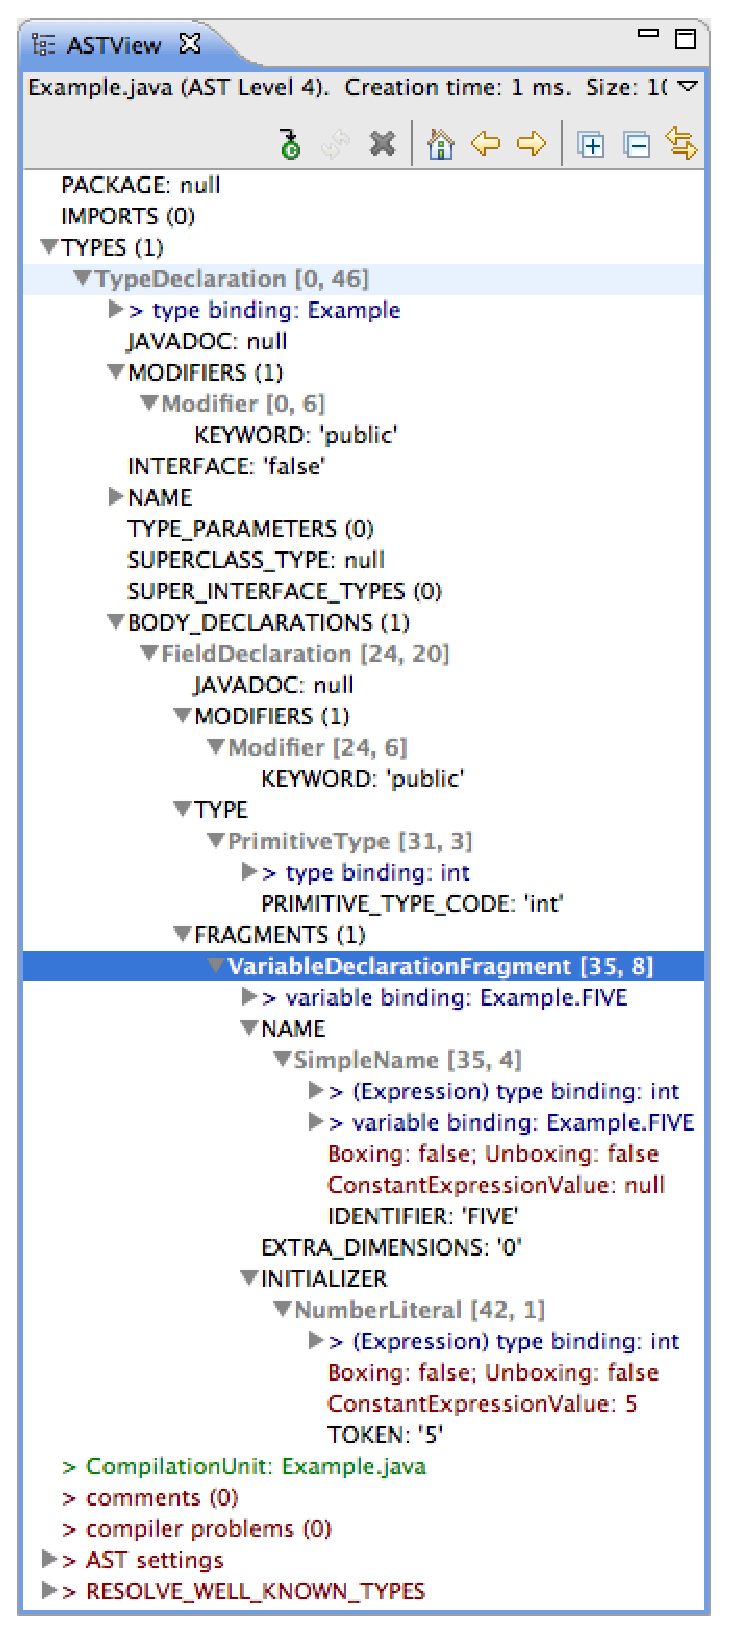
\includegraphics[scale=0.62]{jdt-ast.eps}
%\caption{Visualization of the Eclipse Java Development Tools' abstract syntax
%tree for the following program: \\
%\ \\
%\centerline{\parbox{2in}{\ttt{\noindent public class Example \{ \\
%\hspace*{.2em} public int FIVE = 5; \\
%\}
%}}} \\
%\ \\
%The highlighted node---a \textit{VariableDeclarationFragment}---corresponds to
%the eight-character substring \ttt{FIVE = 5}, which begins with the 36th
%character in the source code.
%}
\caption{Visualization of an AST produced by the Eclipse Java Development Tools
(JDT).\vspace*{-4em}}
\label{fig:jdt-ast}
\end{wrapfigure}

\noindent
\ttt{package} statement, another
contains a list of \ttt{import} statements, and a third contains a list of type
declarations.  A type declaration has several child nodes, which describe
(among other things) its visibility, the name of the class or interface, and
the field/method declarations in its body.  A field declaration has child nodes
describing its visibility, type, and so forth.

Figure~\ref{fig:jdt-ast} shows a visualization of an AST for the following
program:
\vspace*{.5em}

\noindent \ttt{public class Example \{ \\
\hspace*{.2em} public int FIVE = 5; \\
\}
}

\vspace*{.5em}
Notice how deeper levels of the tree describe progressively more fine-grained
syntactic structures.  The root node represents the entire Java source file.
The highlighted node---a \textit{VariableDeclarationFragment}---represents
\ttt{FIVE = 5}, while its child nodes represent its constituent parts: the
identifier \ttt{FIVE} and the numeric literal \ttt{5}.  These are leaf nodes,
since these tokens (like keywords, identifiers, and numeric literals) represent
the smallest syntactic units in the language.

Developers familiar with the HTML or XML DOM (Document Object Model) will find
this structure familiar.  The DOM is effectively an abstract syntax tree for
HTML/XML documents.

Deeper discussions on ASTs can be found in many introductory textbooks on
compiler construction, such as \cite{aho06compilers} and
\cite{torczon11engineering}.  Such books also discuss how parsers are
constructed, including how they can be modified to construct ASTs.

\FloatBarrier

\subsection{Fulfilling the Requirements of Refactoring}
\label{ss:reqs}

%The use of ASTs in refactoring tools is nearly universal.  
%Since refactoring tools analyze and manipulate source code, the primary program
%representation in a refactoring tool is always one that is fairly close to
%source code---generally an abstract syntax tree.  The AST plays an absolutely
%critical role.  It is used for both analysis and transformation, and every
%refactoring makes use of it.

ASTs are not unique to refactoring tools.  They were used in compilers long
before refactoring tools existed.  They are also used in static analysis tools,
prettyprinters, and other tools that analyze source code.  This makes reuse
very tempting: If there is already a compiler for a language, and it contains
an AST, why not reuse it in a refactoring tool?

Unfortunately, an AST designed for use in another context (e.g., a compiler) is
not necessarily suitable for refactoring.  This is because refactoring tools
impose two very significant---and unusual---requirements on their ASTs.

\begin{enumerate}
\item To be useful for refactoring, an AST must accurately and precisely model
the user's source code at a very fine level of detail.  It may even be
necessary to include information about punctuation and comments in order to
refactor code appropriately~\cite{sommerlad08retaining}.
\item It must be possible to map nodes in the AST to locations in the
source code, and vice versa.
\end{enumerate}

To illustrate the first requirement, consider an example from Fortran.  The
Fortran language contains a number of input/output statements.  Two of these
are \textsc{print} and \textsc{write}: the statements \ttt{print *, "X"} and
\ttt{write (*,*) "X"} can be used interchangeably to print the string \ttt{X}
to standard output.  In general, the statement \ttt{print} \textit{fmt}\ttt{,}
\textit{expr} is equivalent to the statement \ttt{write (*,
}\textit{fmt}\ttt{)} \textit{expr}.  Most compilers type check and translate
them identically.  So, a compiler may choose to represent \textsc{print}
statements as \textsc{write} statements in its AST.  The GNU Fortran compiler
does this, for example.  However, the ability to convert \textsc{print}
statements to \textsc{write} statements actually makes for a useful
refactoring.  (Consider a program that uses \textsc{print} statements to write
to standard output, but the programmer later needs to use \textsc{write}
statements to write to a file instead.) To implement this refactoring, a
refactoring tool needs to be able to distinguish \textsc{print} statements from
\textsc{write} statements---a difficult task if they are represented
identically in the AST.

To explain the second requirement---that it must be possible to map nodes in
the AST to locations in the source code, and vice versa---recall that many
refactorings are initiated only after the user selects a range of source code
in a text editor.  Usually, this selection is represented by two numbers: the
\textit{offset} of the starting character and the \textit{length} of the
selection.  In the simple Java program whose AST is shown in
Figure~\ref{fig:jdt-ast}, the substring \ttt{FIVE = 5} is eight characters long
and begins with the 36th character in the source code (offset 35, assuming the
first character is considered to be at offset 0).  If the user selects the text
\ttt{FIVE = 5} in the text editor, it must be easy to determine that this
corresponds to the \textit{VariableDeclarationFragment} node in the AST.


\subsection{Mutable vs.\ Immutable ASTs}
\label{ss:manip}

There are two main variants of abstract syntax tree:
mutable and immutable. A mutable tree has nodes that can be easily added, 
changed, or deleted from the tree. These trees are often used internally by
compilers. For example, a compiler might determine that
\ttt{a~=~b*1} can be simplified to \ttt{a~=~b}, and then change the AST 
accordingly.

At first, this seems like a reasonable mechanism for refactoring tools to use
as well.  To remove a field declaration from a program, simply delete its
\textit{FieldDeclaration} node from the AST (along with all its children).  To
change the name of \ttt{FIVE}, change the contents of its
\textit{SimpleNameNode} in the AST.  Of course, some mechanism is needed to
prettyprint the modified AST, so these changes can be translated back into
source code, but that is relatively straightforward to implement.

Mutable ASTs are simple to understand and allow code for specific refactorings
to be very short. Performing refactorings on source code is conceptually
identical to changing the AST itself. This can greatly lower the bar for 
designing refactorings. However, mutable ASTs introduce a host of problems when
used in a large API:

\begin{itemize}
\item \textit{AST nodes contain source location information.}  After the
structure of the AST is changed, what does the source location information in
each node represent: the ``old'' source location (in the original code) or the
``new'' location (after it has been modified)?  If it represents the old
location, what should the source location be when new nodes are inserted into
the tree?  If it represents the new location, then every time a change is made
to the tree, source location information must be updated for every node in the
tree, which may be expensive \dots or else a clever implementation (e.g.,
computation from relative offsets) must be used instead.
\item \textit{AST nodes may be removed from the tree, leaving them orphaned.}
Suppose a client traverses the AST, storing pointers to some ``interesting''
nodes in a collection.  Then, an ancestor of one of those nodes is removed from
the AST.  This will leave the client in a difficult-to-debug situation where
his collection contains pointers to nodes that no longer exist in the AST.
\item \textit{Semantic information may be invalidated.}  Refactorings often
need to determine, for a particular use of a variable, what declaration that
use corresponds to.  For example, in Java, if a field and a local variable were
both named \ttt{x}, then in the expression \ttt{this.x = x}, the first \ttt{x}
would refer to the field, while the second would refer to the local variable.
However, if the local variable declaration were removed, the second \ttt{x}
would refer to the field instead.  This can be confusing to clients, since
information collected about the program at one point in time may no longer be
true after the tree's structure changes.
\item \textit{It may be possible to mutate the AST so that it does not
represent a legal program.}  It might even be possible to mutate the AST so
that it is no longer a tree at all.  In Java, classes can contain other
classes.  What happens if a client tries to make a class an inner class of
itself?  (This could turn the tree into a cyclic graph.)  The API for modifying
the AST's structure could try to prevent such things, but attempting to detect
and prevent every possible mistake would be difficult and potentially
expensive.
\item \textit{Mutability can be problematic in multithreaded code.}
\end{itemize}

%TODO work on this preprocessor stuff some more
%Maybe move to a different place?
\subsection{Preprocessors}
Preprocessors (such as the C preprocessor and M4), don't interfere with the ASTs
used by compilers. In most cases, the preprocessing is performed first, and the
output thereof is used to construct the AST. The lexer/parser requires no 
knowledge of the fact that the text was preprocessed.

Refactorings, however, are complicated by the C preprocessor. The grammar of 
preprocessor directives doesn't take into account C syntax, and can't be easily
represented in the C AST. This is the subject of Garrido's entire Ph.D.~thesis~%
\cite{garrido05program}. The compiler's method of preprocessing before parsing
can't be used, because the unpreprocessed text is what must be edited. The 
refactoring too must be able to parse, analyze, and transform code \textit{
with embedded preprocessor directives.}

The topic of refactoring preprocessed code will not be treated in detail here,
but suffice it to say that a compiler's AST will almost certainly be inadequate.
For more details, see Garrido~\cite{garrido2013} and Overbey et al.~\cite{wrt2009}.

\section{Solution}

\textit{Use a parser for the language being refactored to construct an
\textup{abstract syntax tree}, or \textup{AST}.  Make the AST
\textup{immutable}---i.e., its structure cannot be changed---but provide
\textup{source mapping} information so that every node in the AST can be mapped
to a particular substring of the original source code. Treat the source code
as a string, and use the source code location information from the AST to
add, replace, and delete substrings.}

\subsection{Immutability}
As seen in Section 3.4, mutability introduces a host of problems to ASTs. Mutable ASTs were used in the original Smalltalk Refactoring
Browser~\cite{roberts97refactoring}, as well as in
CRefactory~\cite{garrido05program} and Photran~\cite{sle2008}.  Many compilers
use mutable ASTs internally.  However, these tools have one thing in common:
the mutable AST is not accessible via any public API.  It is intended for
internal use only, by those tools' developers who should be better equipped to handle all of
the caveats.

Guidelines for API design are discussed in detail in Jaroslav Tulach's
\textit{Practical API Design}~\cite{tulach08practical}.  A presentation by
Joshua Bloch~\cite{bloch} offers excellent advice as well.  Both authors
suggest minimizing the amount of mutability in an API.  Immutable objects tend
to have simpler interfaces, and they are thread-safe.  Both authors also
emphasize that APIs should be easy to learn (even for programmers who do not
read all of the API documentation) and difficult for clients to misuse. Mutable
ASTs have the advantage of ease-of-learning, but have have all the disadvantages
listed above. They can be valid solutions for simpler refactorings or projects
developed by a small team of people, but become problematic when used for 
nontrivial refactorings or for a public API. For a general, public refactoring
API, immutable trees are much more robust.


\subsection{Source Mapping}

As discussed in Section 3.3, it must be possible to map nodes in the AST to
locations in the source code, and vice versa. The easiest way to map AST nodes to source locations is to store source
location information in the AST nodes themselves.  Again, consider the JDT AST
shown in Figure~\ref{fig:jdt-ast}, and note the numbers in square brackets.
The highlighted node is displayed as ``VariableDeclarationFragment [35, 8]'':
this AST node corresponds to the eight-character string beginning at offset 35
(\ttt{FIVE = 5}).  Its child node corresponding to the identifier \ttt{FIVE} is
attributed with the offset-length pair [35, 4], while the numeric literal
\ttt{5}'s source location is [42, 1].

Now, consider what happens when a user selects text in the text editor.  This
can be represented as an offset-length pair.  When source location information
is available for every AST node, it becomes fairly easy to determine what
syntactic the text selection corresponds to: simply
walk the tree, searching for a node whose source location aligns with the
user's selection.

Since AST nodes at deeper levels of the tree represent finer-grained syntactic
constructs than their ancestor nodes, ASTs with source location information
typically exhibit a nice property: the source location of a child node will
always be contained within the source location of its parent.  This property
can be used to expedite searches based on source location information.  For
example, if a particular node corresponds to the source location [35, 8], and
you are searching offset 63, then the desired node cannot possibly be a
descendent of that node.


\subsection{Using Immutable ASTs for Source Code Manipulation}
\label{ss:manip}

The ultimate goal of a refactoring tool is to modify the user's source code.
When ASTs are immutable, this cannot be done by modifying the structure of the
AST.  Instead, it is done differently: \textit{Treat the source code as a
string, and use the source location information in the AST to add, replace, and
delete substrings.}

As an example, consider deleting a field declaration.  In a mutable AST, you
would simply remove the \textit{FieldDeclaration} node from the AST.  With an
immutable AST, you would retrieve the source location mapping from the
\textit{FieldDeclaration} node, and then remove that substring from the source
file.

In implementation, the code for removing a field declaration using a mutable
AST would probably be something like \textit{field.removeFromTree()}.  The code
for doing the same with an immutable AST would be something like
\textit{sourceCode.deleteSubstring(field.getOffset(), field.getLength())}.

The situation gets a bit worse when changes are made to nested constructs.
Recall the example from Section~\ref{sec:Problem}, which reversed conditionals 
of \textit{if} statements. After the addition of the \textit{not} to the 
condition, the offset of the body is different. Consider a somewhat simplified 
example. Pictorially:

\begin{center}
\jb{i}\jb{f}\jb{(}\jb{1}\jb{)}\jb{ }%
\jb{s}\jb{(}\jb{)}\jb{;}\jb{ }%
\jb{e}\jb{l}\jb{s}\jb{e}\jb{ }%
\jb{b}\jb{(}\jb{)}\jb{;}\\
\lb{\,}\kb{0}\kb{1}\kb{2}\kb{3}\kb{4}\kb{5}\kb{6}\kb{7}\kb{8}\lb{9}%
\lb{10}\lb{11}\lb{12}\lb{13}\lb{14}\lb{15}\lb{16}\lb{17}\lb{18}\lb{19}\\
$\Downarrow$ \rule[-0.5em]{0pt}{1.2em} \\
\jb{i}\jb{f}\jb{(}\jb{!}\jb{1}\jb{)}\jb{ }%
\jb{b}\jb{(}\jb{)}\jb{;}\jb{ }%
\jb{e}\jb{l}\jb{s}\jb{e}\jb{ }%
\jb{s}\jb{(}\jb{)}\jb{;}\\
\lb{\,}\kb{0}\kb{1}\kb{2}\kb{3}\kb{4}\kb{5}\kb{6}\kb{7}\kb{8}\lb{9}%
\lb{10}\lb{11}\lb{12}\lb{13}\lb{14}\lb{15}\lb{16}\lb{17}\lb{18}\lb{19}\lb{20}\\
\end{center}

\noindent
The body of the first \textit{if} statement begins at offset~6 in the original
code.  But after interchanging the body statements, the body of
the inner \textit{if} statement is shifted to offset~7. This must be taken into
account when the bodies of the \textit{if} and \textit{else} are switched.

%Likewise, if braces were added to the inner \textit{if} statement first, then
%this would shift the location of the closing brace for the outer \textit{if}
%statement.
In other words, when refactorings affect nested language constructs,
offset/length computations can become complex, since the edits for one
construct may interact with the edits for another construct.

So, manipulating source code using a mutable AST is simpler, and it more
directly expresses the programmer's intention.  Manipulating source code using
offset/length information leads to ugly client code.  The client code can
easily become littered with variables holding character offsets and methods
that perform intricate string manipulations.

In their discussions of API design, Bloch submits that it should be ``easy to
read and maintain code that uses [the API]''~\cite{bloch}, and Tulach notes the
advantages of APIs where the clients ``don't describe step-by-step what they
want your API to do.  Rather, they `declare' what they want to have happen and
then rely on your API to do it\dots''~\cite[p.~225]{tulach08practical}.

So, is it possible to provide a cleaner source manipulation API, while still
using an immutable AST?  It is, and there are two main variants that allow
for this.


\section{Variants}

\begin{itemize}

    \item Functional: \textit{Work with the ASTs in a functional style, where every edit
        returns a new AST.} So, a call to field.removeFromTree() would not
        change the existing AST, but rather it would return a new AST that has
        the given field omitted. When dealing with immutable data structures,
        functional programming may often be the natural solution. However,
        in the case of ASTs, a functional style risks reintroducing many of 
        the problems inherent to mutable trees. File location of nodes may
        be disrupted in the new tree, pointers to nodes in the original tree may
        be rendered 
        irrelevant, semantic information may be invalidated, etc. Those are in
        addition to the difficulties of functional programming, such as memory
        consumption and copying, especially with very large ASTs. This is
        a valid refactoring API design pattern, but any implementation using 
        this variant must carefully consider these problems.

    \item Rewriter: \textit{Provide an API that allows clients to specify what changes
        they want to make in terms of AST nodes.}  This API can then translate these into string edits.  For example, an API might offer a \textit{Rewriter} 
class. The client would inform the \textit{Rewriter} that it wants to 
effectively delete a particular \textit{FieldDeclaration} node from the AST:
\textit{rewriter.delete(field)}.  When it is ready to manipulate the source
code, it delegates this task to the rewriter:
\textit{rewriter.rewrite(sourceCode)}.  This allows multiple edits to be made 
without conflicting with each other. This is illustrated in
Figure~\ref{fig:seq-diagram}.  The Eclipse Java and C/C++ Development
Tools~\cite{cdt-refactoring} take this approach (with slightly different class
and method names).

\begin{figure}[!bt]
\begin{center}
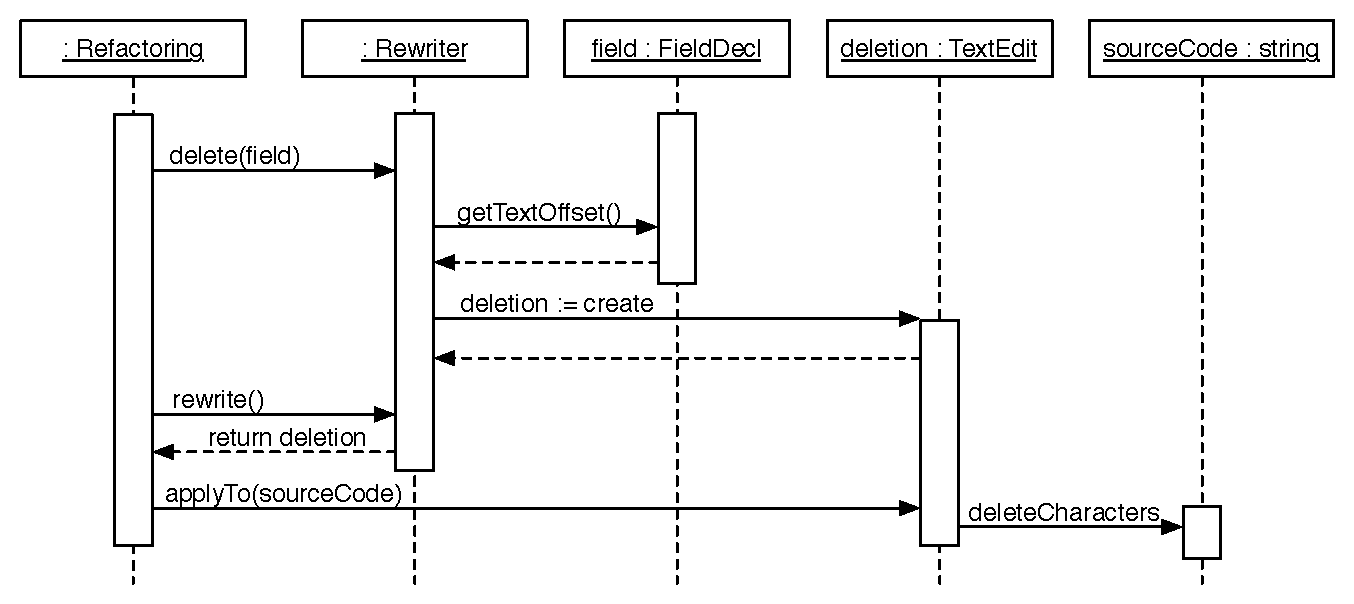
\includegraphics[width=.9\textwidth]{seq-diagram.eps}
\end{center}
\caption{Sequence diagram illustrating use of a Rewriter to modify source code.}
\label{fig:seq-diagram}
\end{figure}

\end{itemize}

\section{Known Uses}

Immutable, source-mapped ASTs are used by the Eclipse Java Development Tools
(JDT) and C/C++ Development Tools (CDT), as well as the Scala IDE for Eclipse,
the Microsoft ``Roslyn'' Community Technology Preview (CTP), Clang, and the
original refactoring engine in Apple Xcode.  However, while all use immutable
ASTs with source mapping information, the actual rewriting APIs vary
substantially.  

Both Clang and the original refactoring engine in Xcode~3.0 modify source code
using offset-length information directly.  Notably, Clang offers a
\textit{RewriteRope} class---essentially, a custom string class that allows for
efficient mid-string insertions and
deletions\footnote{RewriteRope Class Reference: \url{http://clang.llvm.org/doxygen/classclang_1_1RewriteRope.html}}.
(It uses a B-tree structure inspired by, but not identical to, that described
in the original paper on Ropes~\cite{boehm95ropes}.)
 
The Eclipse Platform is designed to be language-independent; individual
plug-ins like JDT and CDT determine what languages it supports.  The Eclipse
Platform includes a component called the Eclipse Language Toolkit
(LTK)~\cite{ltk}.  which provides (among other things) a language-independent
API for manipulating text files using offset/length information.  Specifically,
\textit{TextEdit} objects describe individual changes (like ``delete three
characters starting at offset 462''), and many such changes are aggregated into
a single \textit{Change} object that represents the net effect of a
refactoring.  Of course, the LTK provides the infrastructure necessary to apply
\textit{Change} objects, writing the modifications to disk, as well as to undo
those changes at a later point in time.

Eclipse JDT provides a class (\textit{ASTRewrite}\footnote{\url{http://help.eclipse.org/kepler/topic/org.eclipse.jdt.doc.isv/reference/api/org/eclipse/jdt/core/dom/rewrite/ASTRewrite.html}}) that allows the programmer
to specify modifications in terms of Java AST nodes, and then translates those
changes into an LTK \textit{TextEdit} object.  Eclipse CDT's refactoring engine
is based on JDT's and follows a similar design; it offers its own version of
\textit{ASTRewrite}~\cite{cdt-refactoring}.

Refactoring support in the Scala IDE for
Eclipse\footnote{\url{http://scala-refactoring.org},
\url{http://scala-ide.org/}} takes a functional approach, implementing
refactorings as tree transformations.  Source generation is handled separately:
one printer uses position information to retain the formatting of the original
code, while another pretty-prints new nodes that were added to the
AST~\cite{stocker10scala}.

Microsoft's ``Roslyn'' CTP takes a functional approach, where imperative
methods on AST nodes do not modify the AST but rather return a new
AST~\cite{vogel12roslyn}.  Since a na\"{i}ve implementation could make this
prohibitively expensive, the Roslyn team devised an implementation that
they call \textit{red-green trees} (named after the colors of the
whiteboard markers that were used during the design
meeting)~\cite{lippert12persistence}.  Essentially, the AST exposed via the API
(the ``red tree'') is a fa\c{c}ade for a different, internal tree (the ``green
tree''); the implementation attempts to reuse existing AST nodes whenever
possible (which is possible since all nodes are immutable).

% TODO: Preprocessor complications
% TODO: Example code?

\section{Example}
We created a plugin for Eclipse that exhibits the \emph{Rewriter} variant of this
pattern\footnote{GitHub Repository: \url{https://github.com/aggrand/reverse-conditional}}. It performs the \emph{reverse conditional} refactoring described 
earlier in both JDT and CDT. The pattern is most visible in the plugin's
swapStatements method, Figure~\ref{fig:swapStatements}, which swaps the 
branches of the \emph{if} statement.

As can be seen, the AST provides simple methods to retrieve individual nodes as
objects. The desired changes are then described to the \emph{rewriter}, which
doesn't make any actual changes until all edits are collected. In the case of
this refactoring, the only other change is the negation of the conditional 
expression, which is performed in a similar manner, replacing the existing
expression with a negated one. 

The pattern is similar in both CDT and JDT, to the extent that the plugin is
structured identically, with slightly different class names in each.

\begin{figure}
\begin{center}
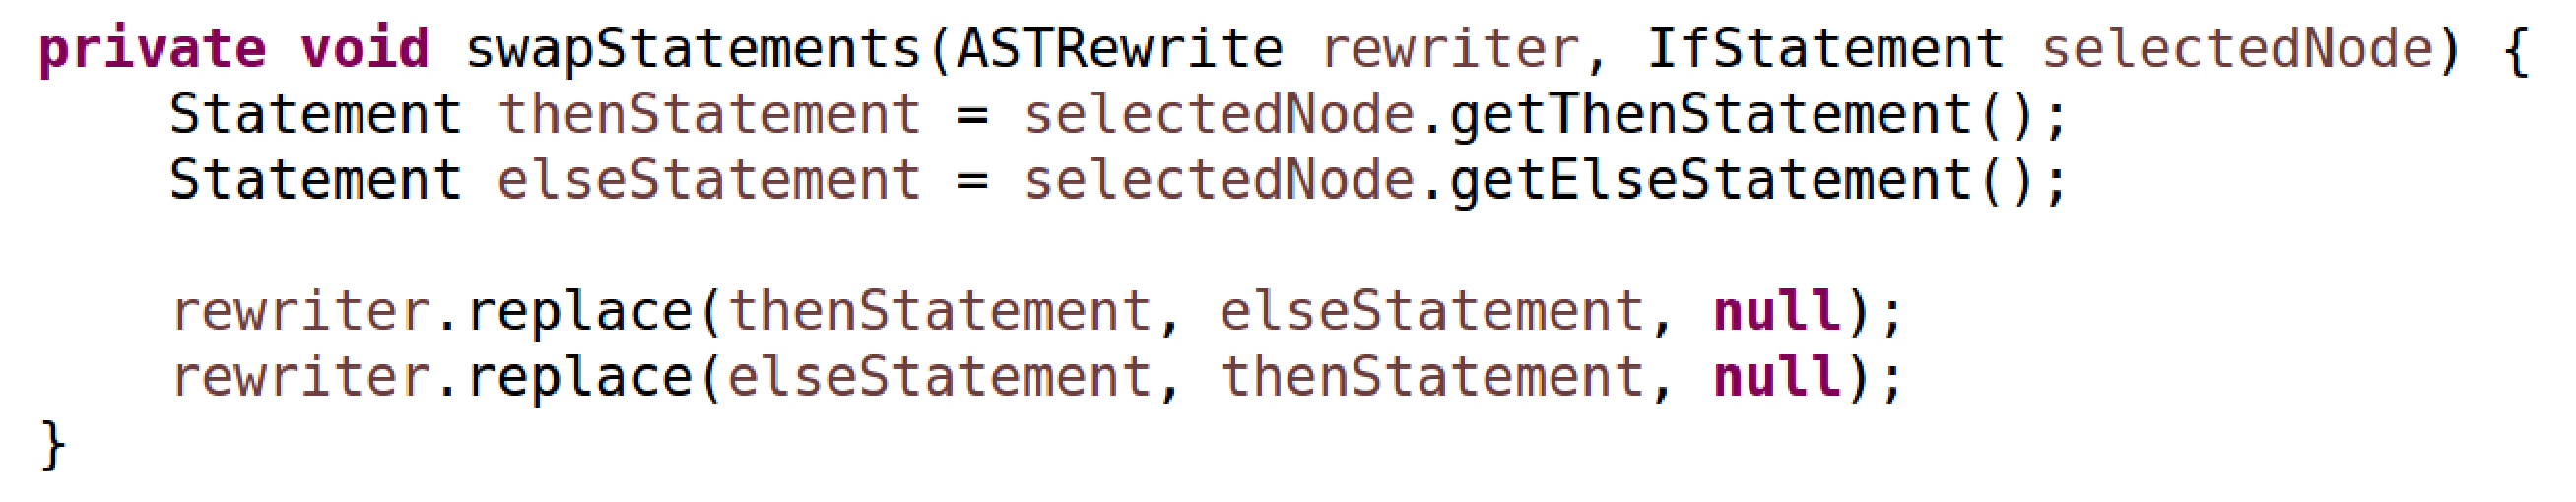
\includegraphics[scale=0.30]{swapStatements.eps}
\caption{The \emph{swapStatements} method.\vspace*{-4em}}
\label{fig:swapStatements}
\end{center}
\end{figure}

\section*{Acknowledgments}
This material is based upon work supported by the National Science Foundation
under Grant No.~CCF-1217271.  The author would like to thank Peter Sommerlad,
who shepherded this pattern, as well as the members of Workshop~000001 at
PLoP~2013: Filipe Correia, Dibyendu Goswami, Joshua Kerievsky, Juan Reza, and
Russ Rubis.  Their feedback was immensely helpful.

\bibliographystyle{acmlarge}
\bibliography{paper}

% History dates
%\received{February 2009}{July 2009}{October 2009}

\end{document}
